\appendix
\subsection{Source Code Repository}

The complete source code developed for this thesis is available in a public GitHub repository. The repository contains the GStreamer pipelines for all configurations, the logging implemented with element probes for per stage timestamps, the measurement and analysis scripts, and the configuration files used across the experiments. Graphs for each measurement attribute for each test T1 to T6 and C1 to C9. A README.md file at the root of the repository describes the structure of the repository and explains how to navigate it and run the pipeline, so that the measurements can be reproduced. The repository is available at the following address:

\begin{center}
\url{https://github.com/einartmy01/Masterthesis}
\end{center}

\subsection{AI Declaration}
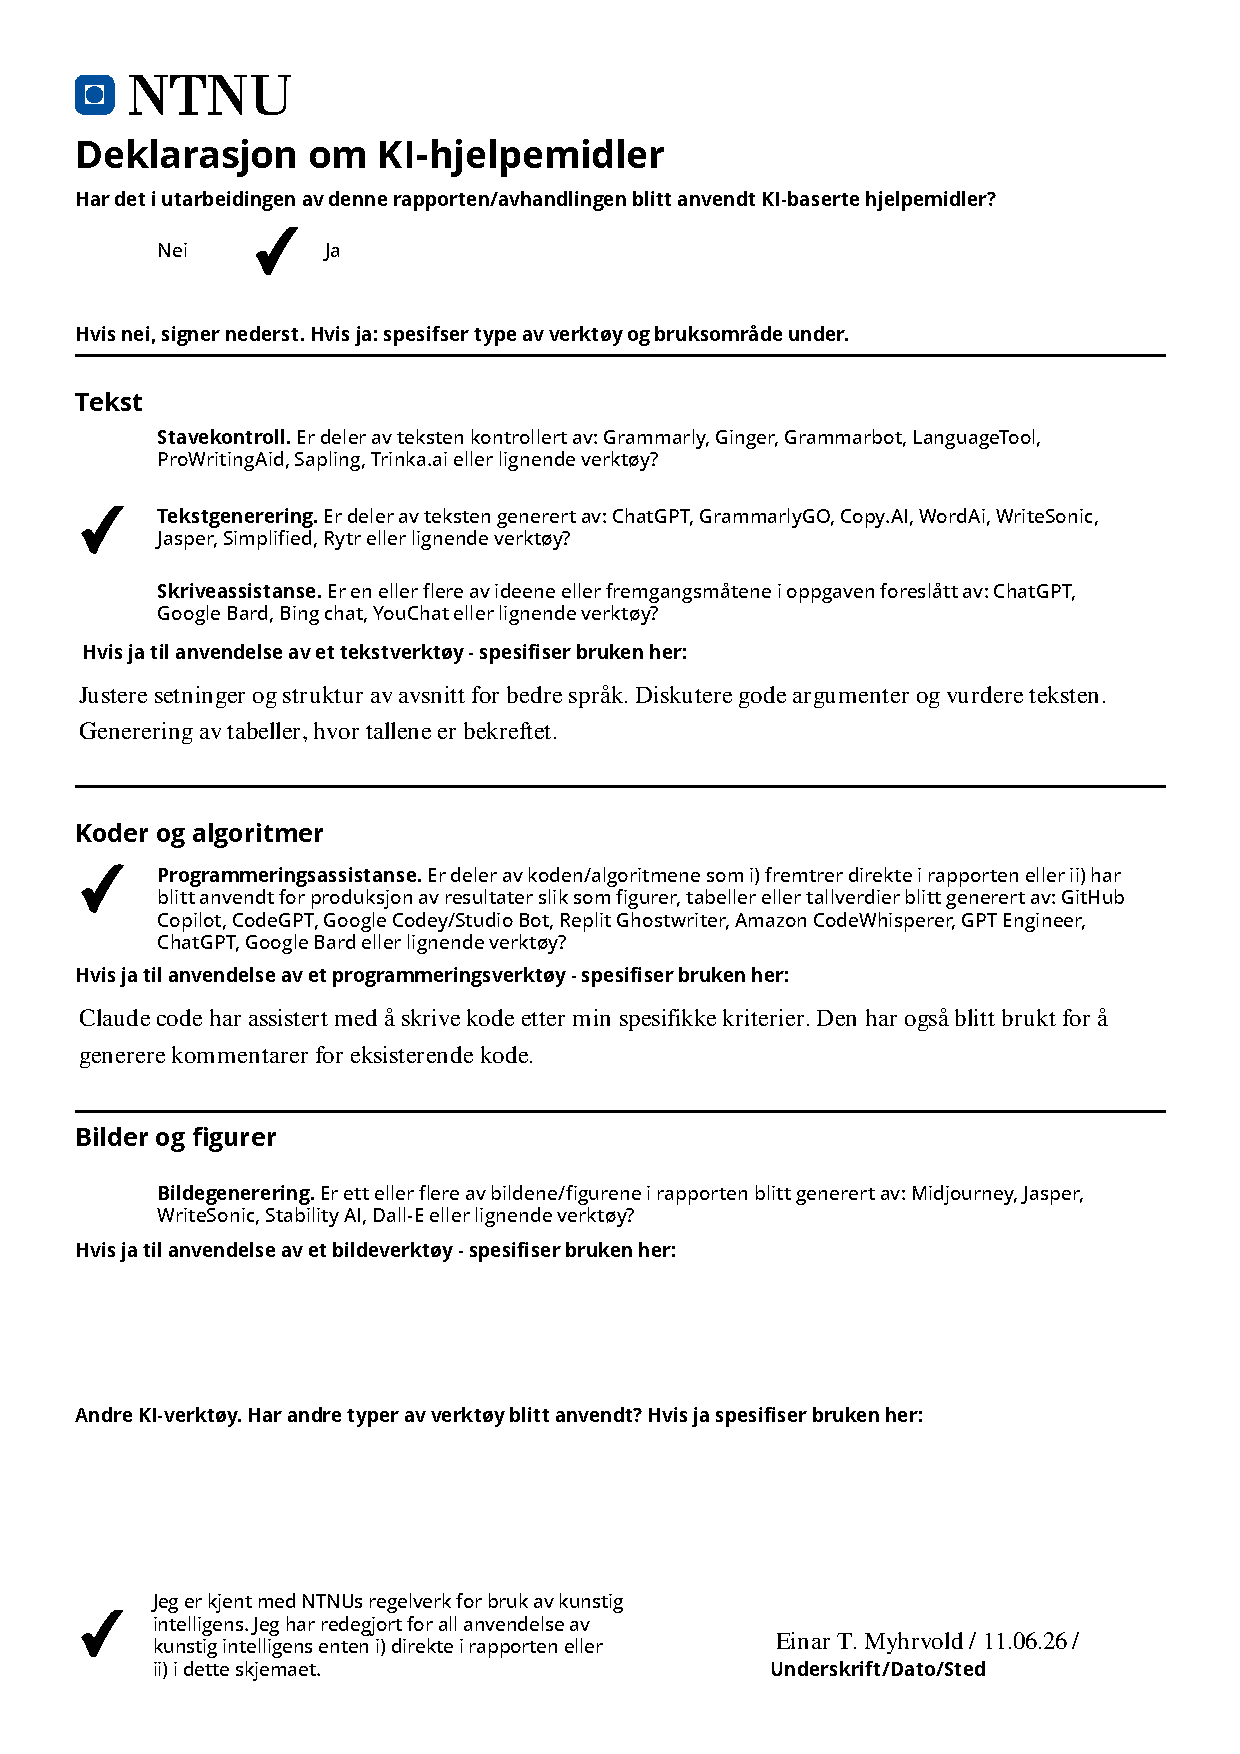
\includepdf[pages=-]{Appendices/NTNU_AI_Declaration.pdf}